\documentclass[sutton_barto_notes.tex]{subfiles}

\begin{document}

\newpage
\section{Monte Carlo Methods}

MC, is for estimating value functions and discovering optimal policies. Unlike methods in previous chapters, MC does not use complete knowledge of the environment. MC only requires \textit{experience} - sample sequences of states, actions and rewards from actual or simulated interaction with an environment. That is, MC is a \textbf{model-free} learning method.

MC is based on averaging complete sample returns. Since we are considering sampling returns, we define MC only for episodic tasks (in this book) \footnote{We can never sample an actual return value in continuous tasks. We may get around by using artificial time horizon, or TD (with eligibility traces); however, all these incur bias. see \url{https://datascience.stackexchange.com/a/77789/137431}}. Once an episode ends, the value estimates and policies change. MC is thus a episode-by-episode update, not a step-by-step (online) update.

The procedure of MC is similar to DP: prediction problem (finding $v_\pi$ and $q_\pi$) -> policy improvement -> control problem (solve by GPI). Except that, in DP, we compute value functions based on model, here we learn value functions from sample returns.

\subsection{Monte Carlo Prediction}

To learn $v_\pi$, we average the returns observed after visits to that state. The more returns are observed, the more closer to the expected value (recall the Law of Large Numbers). Each occurrence of $s$ in an episode is called a \textit{visit} to $s$. First-visit to $s$ is the first time $s$ is visited in an episode.

Note that in the following algorithms, we compute the returns backwards from timestep $T-1$ to $0$.

\begin{tcolorbox}[width=1.1\textwidth,title={First-visit MC prediction, for estimating $V \approx v_\pi$}]
Input: policy $\pi$ (to be evaluated)
Initialize:

$\quad V(s) \in \R$, arbitrarily.
$Returns(s) \leftarrow$ an empty list, $\forall s \in \mathcal{S}$

Loop forever (for each episode):

$\quad$Generate an episode following $\pi : S_0, A_0, R_1, S_1, A_1, R_2, ..., S_{T-1}, A_{T-1}, R_T$

$\quad G \leftarrow 0$

$\quad$Loop for each step of episode, $t = T-1, T-2, ..., 0:$

$\quad\quad G \leftarrow \gamma G + R_{t+1}$

$\quad\quad$if $S_t$ not appears in $S_0, S_1, ..., S_{t-1}:$

$\quad\quad\quad$Append $G$ to $Returns(S_t)$

$\quad\quad\quad V(S_t) \leftarrow$ average($Returns(s)$)
\end{tcolorbox}

\begin{tcolorbox}[width=1.1\textwidth,title={Every-visit MC prediction, for estimating $V \approx v_\pi$}]
Input: policy $\pi$ (to be evaluated)
Initialize:

$\quad V(s) \in \R$, arbitrarily.
$Returns(s) \leftarrow$ an empty list, $\forall s \in \mathcal{S}$

Loop forever (for each episode):

$\quad$Generate an episode following $\pi : S_0, A_0, R_1, S_1, A_1, R_2, ..., S_{T-1}, A_{T-1}, R_T$

$\quad G \leftarrow 0$

$\quad$Loop for each step of episode, $t = T-1, T-2, ..., 0:$

$\quad\quad G \leftarrow \gamma G + R_{t+1}$

$\quad\quad$Append $G$ to $Returns(S_t)$

$\quad\quad V(S_t) \leftarrow$ average($Returns(s)$)
\end{tcolorbox}

The first-visit MC method estimates $v_\pi (s)$ as the average of the returns following first visit to $s$.

The every-visit MC method averages the returns following all visits to $s$. This method extends more naturally to function approximation (chap 9) and eligibility traces (chap 12).

Advantage of MC over DP: (1) no need the model (i.e. the transition dynamics); (2) can work with sample episodes \textit{alone}; (3) can estimate the target state only while ignoring all other states (MC does not bootstrap, meaning each state estimation is independent of other states).

\subsection{Monte Carlo Estimation of Action Values}

When without a model, $v(s)$ along cannot determine $\pi$; in this case, $q(s,a)$ is more useful. Thus, one of MC goals is to estimate $q_*$.

The only problem is that many $(s,a)$ pairs may never be visited. For example, if we have a deterministic policy we only get one action per state (the one that the policy favor). Hence, we only observe returns for one action. This is a problem of \textbf{maintaining exploration}.
One way to solve this is exploring starts.
\textit{exploring starts}: assume episodes start in a $(s,a)$ pair, and that every pair has a nonzero probability to be selected at the start. (This is sometimes useful). A more common way to go about it, is to only consider stochastic policies where the probability of every action in every state is not 0.

\begin{tcolorbox}[width=1.1\textwidth,title={MC Exploring Starts, for estimating $V \approx v_\pi$}]
Initialize:

$\quad \pi(s) \in \mathcal{A}(s)$ (arbitrarily), $\forall s in \mathcal{S}$

$\quad Q(s,a) \in \R$ (arbitrarily), $\forall s \in \mathcal{S}, a \in \mathcal{A}(s)$

$\quad Returns(s,a) \leftarrow$ empty list, $\forall s \in \mathcal{S}, a \in \mathcal{A}(s)$

Loop forever (for each episode):

$\quad$ Choose a random $(S_0, A_0)$ pair s.t. all pairs have nonzero probability

$\quad$ Generate an episode(SAR trajectory) from $(S_0, A_0)$, following $\pi$

$\quad G \leftarrow 0$

$\quad$ Loop for each step of episode, $t = T-1, T-2, ..., 0$:

$\quad\quad G\leftarrow \gamma G + R_{t+1}$

$\quad\quad$ if $(S_t, A_t)$ pair not in the episode:

$\quad\quad\quad$ Append $G$ to $Returns(S_t, A_t)$

$\quad\quad\quad Q(S_t, A_t) \leftarrow$ average$(Returns(S_t, A_t))$

$\quad\quad\quad \pi(S_t) \leftarrow \argmax_a Q(S_t, a)$

\end{tcolorbox}

We use exploring start for evaluating deterministic policy, and $\epsilon$-greedy for evaluating stochastic policy.

\subsection{Monte Carlo Control}

We now look at how our MC estimation can be used in control. Meaning, to approximate optimal policies.

The idea is to follow generalized policy iteration (GPI), where we will maintain an approximate policy and an approximate value function.
We continuously alter the value function to be a better approximation for the policy, and the policy is continuously improved (see previous chapter).


The policy evaluation part is done exactly as described in the previous chapter (MC Prediction), except that we are evaluating the state-action pair, rather than states.

The policy improvement part is done by taking greedy actions in each state. That is, for any action-value function $q$, and for every state $s$, the greedy policy chooses the action with maximal action-value:
$$ \pi(s) \doteq \argmax_a q(s,a) $$

\subsection{Monte Carlo Control without Exploring Starts}

To make sure that all actions are being selected infinitely often, we must continuously select them.
There are 2 approaches to ensure this — on-policy methods and off-policy methods.

\begin{definition}
\textbf{On-policy methods}: evaluate or improve the policy that is used to make decisions.
\end{definition}
\begin{definition}
\textbf{Off-policy method}: evaluate or improve a policy different from the one used to generate the data (make decisions). The policy being evaluated/improved is \textit{target policy}, and the one generate behavior is \textit{behavior policy}.
\end{definition}

On-policy method is a special case of off-policy method, where policy $\pi_t$ = $\pi_b$.

\begin{definition}
\textbf{soft policy}: $\pi(a|s) > 0\quad \forall s \in \mathcal{S}$ and $\forall a \in \mathcal{A}(s).$
\end{definition}

\begin{definition}
\textbf{$\epsilon$-soft policy}: $\pi(a|s) \geq \frac{\epsilon}{|\mathcal{A}(s)|} \quad \forall s \in \mathcal{S}$ and $\forall a \in \mathcal{A}(s)$ and for some $\epsilon > 0$.
\end{definition}

For example, $\epsilon$-greedy policies are examples of $\epsilon$-soft policies. 
$\epsilon$-soft policy gradually moves closer to a deterministic optimal policy.

\begin{figure}[!h]
  \centering
  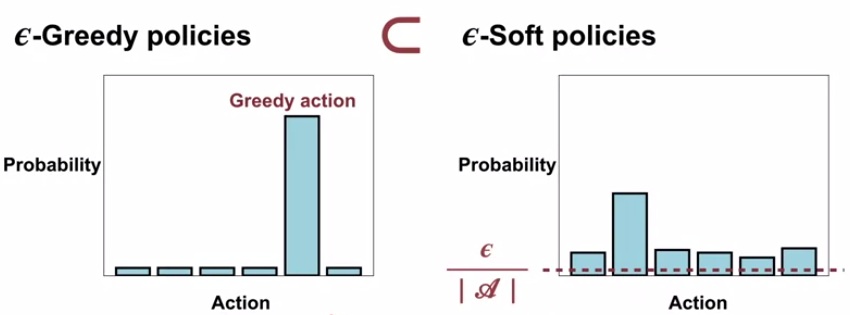
\includegraphics[width=0.6\linewidth]{epsilon-soft.png}
  \label{fig:GPI}
\end{figure}

\begin{tcolorbox}[width=1.1\textwidth,title={On-policy first-visit MC control, estimates $V \approx v_\pi$}]
parameter: small $\epsilon$ > 0

Initialize:

$\quad \pi(s) \leftarrow$ an arbitrary $\epsilon$-soft policy

$\quad Q(s,a) \in \R$ (arbitrarily), $\forall s \in \mathcal{S}, a \in \mathcal{A}(s)$

$\quad Returns(s,a) \leftarrow$ empty list, $\forall s \in \mathcal{S}, a \in \mathcal{A}(s)$

Loop forever (for each episode):

$\quad$Generate an episode(SAR trajectory) following $\pi$

$\quad G \leftarrow 0$

$\quad$Loop for each step of episode, $t = T-1, T-2, ..., 0$:

$\quad\quad G\leftarrow \gamma G + R_{t+1}$

$\quad\quad$if $(S_t, A_t)$ pair not in the episode:

$\quad\quad\quad$Append $G$ to $Returns(S_t, A_t)$

$\quad\quad\quad Q(S_t, A_t) \leftarrow$ average$(Returns(S_t, A_t))$

$\quad\quad\quad A* \leftarrow \argmax_a Q(S_t, a) \quad$ (with ties broken arbitrarily)

$\quad\quad\quad$For all $a \in \mathcal{A}(S_t):$
$\quad\quad\quad\quad$ \begin{equation}
  \pi(a|S_t) \leftarrow
    \begin{cases}
      1 - \epsilon + \epsilon / |\mathcal{A}(S_t)| & \text{if $a = A*$ (greedy)}\\
      \epsilon / |\mathcal{A}(S_t)| & \text{if $a \neq A*$ (non-greedy)}
    \end{cases}       
\end{equation}
\end{tcolorbox}

Soft policies cannot find optimal policy; instead, it can only find optimal $\epsilon$-soft policy because we always give at least $\epsilon / |A|$ probability for each action, which cannot converge to an optimal deterministic policy. On the contrary, exploring start can find optimal policy. However, soft policy can perform generally well so we can abandon exploring start.

The optimal $\epsilon$-soft policy is an $\epsilon$-greedy policy.

\subsection{Off-policy Prediction via Importance Sampling}

Recall the exploration-exploitation dilemma. On-policy learning is actually a compromise: it learns action values ($q$) not for the optimal policy, but for a \textit{near}-optimal policy that still explores. Since they cannot learn a optimal policy while behaving a exploratory policy.

The solution is off-policy: we use two policies, one for leaning optimal-policy, and one for exploration. We use episodes generated from the behavior policy to go and explore the environment, and then use this to update our target policy. We do this to estimate $v_\pi$ and $q_\pi$.

There are other useful applications of off-policy learning, such as learning from demonstration and parallel learning. But facilitating exploration is one of the main motivators.

In the prediction step of GPI, the target and behavior policies are fixed. All we have are episodes following behavior policy $\pi_b$. \textbf{Assumption of \textit{coverage}}: $\pi(a|s) > 0$ implies $b(a|s) > 0$; policy $b$ must be stochastic in states where $b \neq \pi$.

For off-policy learning to work, we need to align policy $\pi$ and policy $b$ through importance sampling.
\begin{definition}
\textbf{Importance sampling}: a method of estimating expected values of one (target) distribution, given samples from another (behavior) distribution.
\end{definition}

We apply importance sampling to off-policy learning by using importance sampling ratio.
\begin{definition}
\textbf{Importance sampling ratio}: weight the returns based on the relative probability of their trajectories occurring under $\pi$ and $b$.
\end{definition}
The probability of the state-action trajectory, from $S_t$, $A_t, S_{t+1}, A_{t+1},...,S_T$ occurring under policy $\pi$ is:
\begin{align*}
& Pr\{A_t, S_{t+1}, A_{t+1}, ..., S_T | S_t, A_{t:T-1} \sim \pi\}\\
& = \pi(A_t|S_t)p(S_{t+1} | S_t, A_t) \pi(A_{t+1} | S_{t+1}) ... p(S_T | S_{T-1}, A_{T-1}) \\
& = \prod_{k=t}^{T-1} \pi(A_k|S_k)p(S_{k+1} | S_k, A_k)
\end{align*}
Thus, the importance sampling ratio is:
$$ \rho_{t:T-1} \doteq \frac{\prod_{k=t}^{T-1} \pi(A_k|S_k)p(S_{k+1} | S_k, A_k)}{\prod_{k=t}^{T-1} b(A_k|S_k)p(S_{k+1} | S_k, A_k)} = \prod_{k=t}^{T-1} \frac{\pi(A_k|S_k)}{b(A_k|S_k)} $$
Note after canceling the transition probabilities, the importance sampling ratio depends only on the two policies and the sequence, not on the MDP.
\begin{align*}
\E_\pi [X] & \doteq \sum_{x \in X} x \pi(x) = \sum_{x \in X} x\pi(x) \frac{b(x)}{b(x)} = \sum_{x \in X} x \underbrace{\frac{\pi(x)}{b(x)}}_{\rho(x)} b(x) \\
& = \sum_{x \in X} \underbrace{x \rho(x)}_{\text{new random var} X} b(x) \\
& = \sum_{x \in X} X b(x)\\
& = \E_b [X \rho(X)]
\end{align*}
$$\E_b[X\rho(x)] = \sum_{x \in X} x \rho(x) b(x) \approx \frac{1}{n}\sum_{i=1}^n x_i \rho_i (x), x_i \sim b\quad \text{(by def of $\E$)}$$
All we have from the behavior policy are returns $G_t$, we can use these returns to estimates $v_b(s) = \E [G_t | S_t = s]$, but not $v_\pi$. To adjust for the difference between $v_b$ and $v_\pi$, we apply importance sampling ratio $\rho$:
$$ v_\pi(s) = \E [ \rho_{t:T-1} G_t | S_t = s] $$

\subsection{Summary}

\begin{itemize}
\item MC advantages over DP: (1) no need of model to learn; (2) MC can be used with simulation or sample models; (3) MC can focus on a small subsets of the states (can just keep visiting target states); (4) less influenced by violations of the Markov property because MC do not bootstrap.
\item MC provide an alternative Policy Evaluation process. They average sample returns instead of using a model to compute $v(s)$.
\item action-value functions can be used to improve the policy without a model.
\item Off-policy prediction: learning the value function of $\pi_{target}$ from data generated by a different $\pi_b$.
\item ordinary importance sampling: unbiased estimates but large(inf) variance.
\item weighted importance sampling: biased estimate with finite variance
\end{itemize}


\subsection{Learning Objectives (UA RL MOOC)}

Lesson 1: Introduction to Monte-Carlo Methods 

1. Understand how Monte-Carlo methods can be used to estimate value functions from sampled interaction 

Because value of a state is the expected return (expected cumulative future discounted reward), and MC estimate the $V(s)$ by averaging the returns from visits to those states. Due to the Law of Large Numbers, the estimated value converges to the true value once there are enough sample returns.


2. Identify problems that can be solved using Monte-Carlo methods 

MC can be used to solve problems that is hard to define a MDP model. For example, we can use MC to solve Blackjack and Soap Bubble problem from the book.

3. Use Monte-Carlo prediction to estimate the value function for a given policy. 

This is a MC prediction problem. We can solve the problem by MC first-visit method, or MC every-visit method.

Lesson 2: Monte-Carlo for Control 

4. Estimate action-value functions using Monte-Carlo 

When there is no model available, we can estimate action values. We can use MC Exploring Start for the problem. Or we can use the same methods for estimating $V(s)$, with MC first-visit/every-visit methods.

5. Understand the importance of maintaining exploration in Monte-Carlo algorithms 

If we don't explore enough, then some $(s,a)$ pairs are never visited. Without enough return, we cannot effectively estimate $q(s,a)$ by averaging.

6. Understand how to use Monte-Carlo methods to implement a GPI algorithm

Policy evaluation is done by averaging enough returns; policy improvement is that $\pi(s) \doteq argmax_a q(s,a)$.

7. Apply Monte-Carlo with exploring starts to solve an MDP 

see Chap 5.2

Lesson 3: Exploration Methods for Monte-Carlo 

8. Understand why exploring starts can be problematic in real problems 

For example, we cannot let a self-driving car to start in all $(s,a)$ situations. Some of them can be dangerous!

9. Describe an alternative exploration method for Monte-Carlo control 

We can use on-policy ($\epsilon-soft$) methods, or off-policy (one behavior policy + one target policy) methods.

Lesson 4: Off-policy learning for prediction 

10. Understand how off-policy learning can help deal with the exploration problem 

Off-policy learning has one policy that is specific to explore the world (and generate behavior), and the other policy is to used the experience to learn.

11. Produce examples of target policies and examples of behavior policies

target policy can be a robotic arm, behavior policy is the expert.

12. Understand importance sampling

Importance sampling is a technique for estimating expected values under one distribution given samples from another. 

13. Use importance sampling to estimate the expected value of a target distribution using samples from a different distribution

$$ \rho_{t:T-1} = \prod_{k=t}^{T-1} \frac{\pi(A_k|S_k)}{b(A_k|S_k)} $$

14. Understand how to use importance sampling to correct returns 

With enough returns, we can lower the variance and eventually return the true value.

15. Understand how to modify the Monte-Carlo prediction algorithm for off-policy learning.

We use importance sampling for off-policy MC.

\end{document}